\documentclass[12pt,fleqn]{article}\usepackage{../common}
\begin{document}
SVD ile Kumeleme

Tekil Deger Ayristirma (Singular Value Decomposition -SVD-) ile bir veri
madenciligi ornegi gorecegiz. Ornek olarak [1] adresinde tarif edilen /
paylasilan zaman serisini kullandik. Serinin tumunu kullanilmadi, ilk 10
noktasini aldik, ve grafige bakinca iki tane ana seri turu oldugunu
goruyoruz.

\lstinputlisting[language=Python]{time1.py}

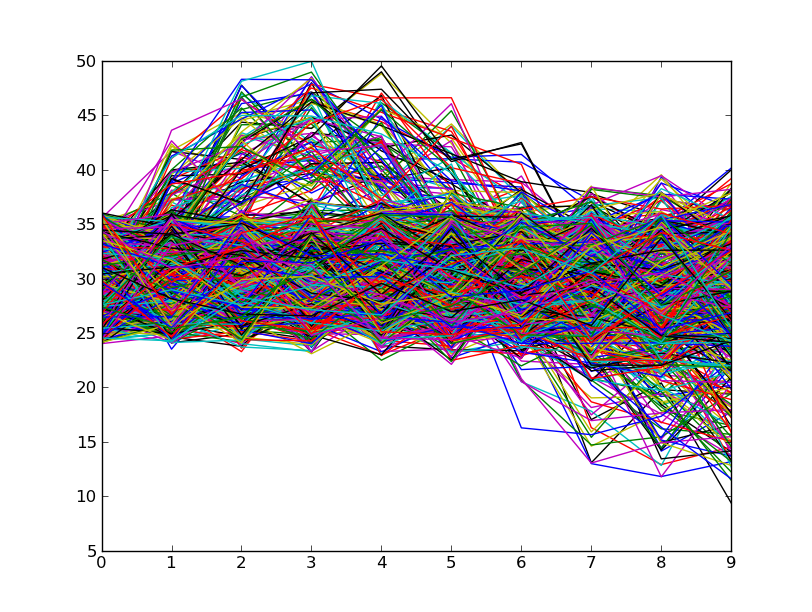
\includegraphics[height=6cm]{data.png}

Peki bu serileri nasil otomatik olarak kumeleyerek bulurduk / birbirinden
ayirtederdik?  {\em Lineer Cebir Ders 29}'da SVD'nin matematigini
isledik. SVD bir matris $A$ uzerinde ayristirma yapar, ve $A$ herhangi
boyutta, turde bir matris olabilir.

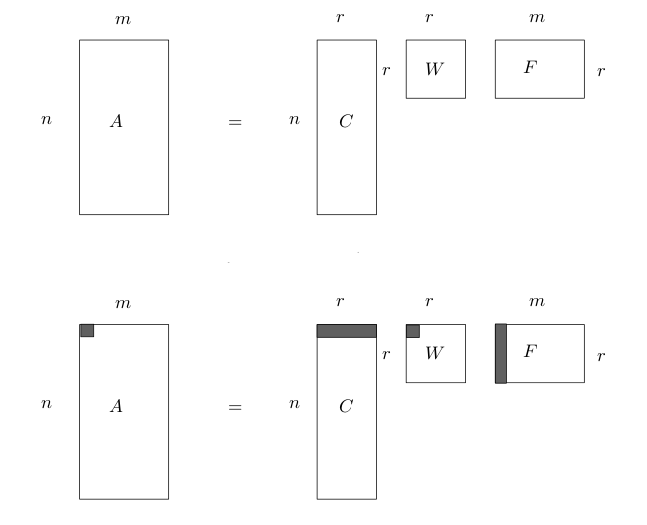
\includegraphics[height=8cm]{svd1.png}

Ayristirma $m \times n$ boyutlu matrisi $A=CWF$ olarak ayristirir, burada
$C$, ana matris ile ayni miktarda satira sahiptir, $F$ ayni miktarda kolona
sahiptir. Ayristirma sonrasi $A$'nin kertesi (rank) $r$ ortaya cikar, eger
tum $A$ kolonlari birbirinden bagimsiz ise, o zaman $r=m$ olacaktir, ama
kolonlarin bazilari mesela ayni olcumu degisik katlarda tekrarliyor ise, o
zaman matriste tekillik vardir, ve bu durumda $r < m$ olur, ve ortadaki $W$
matrisi $r \times r$ oldugu icin beklenenden daha ufak boyutlarda
olabilir. 

Ayrica SVD, $W$ caprazindaki ozdegerleri buyukluk sirasina gore dizer, ve
her ozdegere tekabul eden ozvektorler de ona gore siraya dizilmis
olacaktir, ve SVD tamamlaninca mesela ``en buyuk 10'' ozdegere ait olan
$CWF$ degerlerini alip, digerlerini atmayi da secebiliriz, yani kerte
uzerinden yapilan ``eleme'' ustune bir eleme de kendimiz yapabiliriz. Bu
elemeyi yapabilmemizin mantigi soyle; kucuk ozdegerlerin carptigi
ozvektorlerin nihai toplama daha az etki ettigi soylenebilir, ve bu
``gurultuyu'' elemek sonucu degistirmeyecektir. Ayrica bu elemeyi yaparak
bir tur boyut azaltma (dimensionality reduction) islemini de ayni zamanda
basarmis oluruz.

Ayristirmanin Anlamlari

Bir ayristirmayi degisik sekillerde gormek mumkundur. Bunlardan onemli
birisi cizge bakis acisidir (graph interpretation). Cizge bilindigi gibi
dugumler ve onlar arasindaki ayritlardan (edges) olusur. Bir cizge matris
formunda temsil edilebilir, satir / kolon kesisimi iki dugum arasindaki
ayritin agirligini, ya da varligini (1 ve 0 uzerinden) temsil edecektir. Bu
durumda SVD sonucunda elde edilen $CWF$, bize iki dugum arasi gecisli
(bipartite) cizgeyi, uc dugum arasi gecisli (tripartite) cizgeye cevrilmis
halde geri verir. Ve bu yeni cizgede en fazla $r$ tane gecis noktalari
(waystations) olusmustur, ustte bahsettigimiz eleme ile gecisler daha da
azaltilabilir. 

Simdi, bu gecis noktalarina olan $C$'nin ``baglanma sekli'', ``baglanma
kuvveti'', ek kumeleme basamagi tarafindan kullanilabilir. Bu
``azaltilmis'' gecisin uzerindeki her islem / ona yapilan her referans
kumeleme icin bir ipucudur. Bunu gormek icin ornek zaman serilerinin SVD
sonrasi elde edilen $C$ (ornekte \verb!u!) matrisinin ilk iki kolonunu bile
grafiklemek yeterlidir.

\lstinputlisting[language=Python]{time2.py}

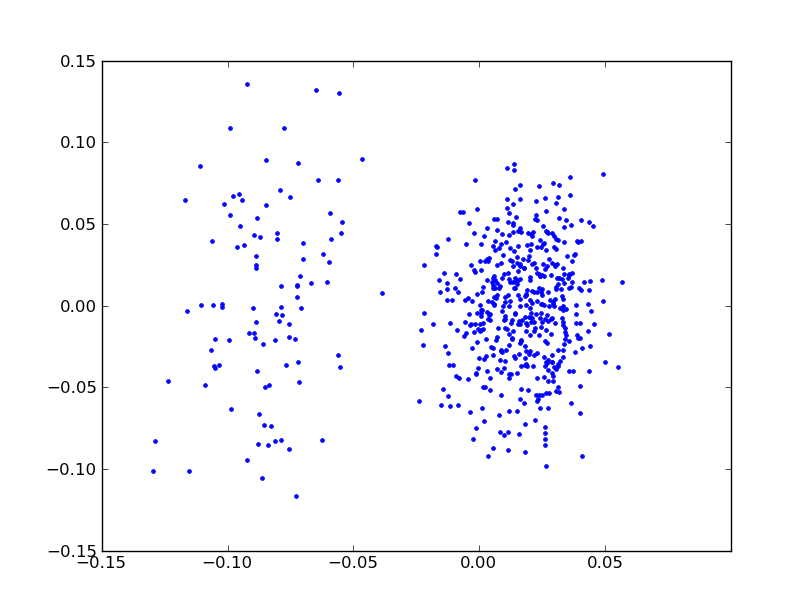
\includegraphics[height=8cm]{2d.png}

Goruldugu gibi net bir sekilde iki tane kume ortaya cikti. Bu kumeler
yazinin basindaki iki ayri zaman serisi obeklerine tekabul ediyorlar. 

O zaman serilerini ayirtetmek icin ne yapariz? Ustteki veriler uzerinde
kmeans isletebilirdik, ya da kabaca bakiyoruz, dikey olarak \verb!-0.025!
seviyesinde bir cizgi ayirac olarak gorulebilir. Numpy filtreleme teknigi

\begin{lstlisting}[language=Python]
u[:,0] < -0.025
\end{lstlisting}

bize ana veri uzerinde uygulanabilecek \verb!True! ve \verb!False!
degerleri verir, bunlari alarak ana veriye filtrele olarak uygulariz,

\begin{lstlisting}[language=Python]
data[u[:,0] < -0.025]
\end{lstlisting}

ve mesela birinci kumeye ait zaman serilerini bulabiliriz. 

Kontrol etmek icin ilk 3 kolonun degerlerini uc boyutta grafikleyelim.

\lstinputlisting[language=Python]{time3.py}

Yine iki tane kume oldugunu goruyoruz. 

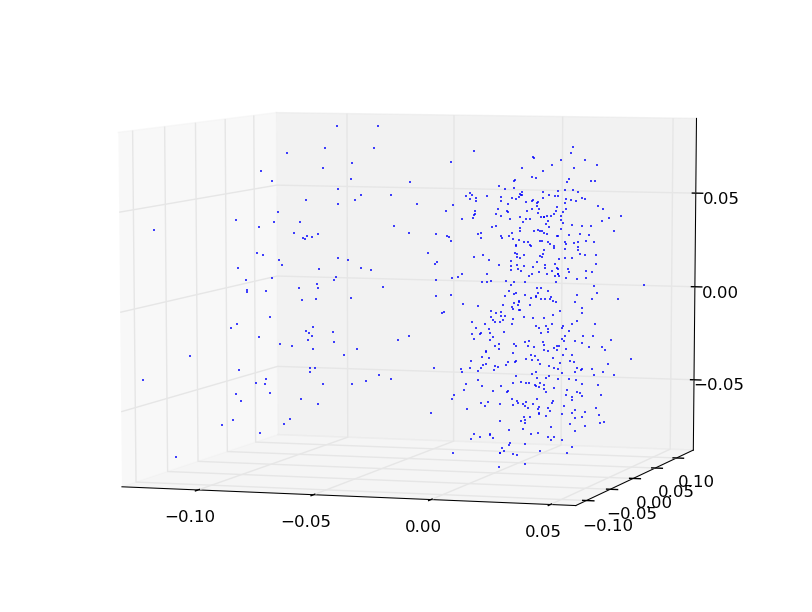
\includegraphics[height=8cm]{3d.png}

Simdi biraz daha degisik bir probleme bakalim, bu sefer bir grup kelimeyi
birbirlerine benzerlikleri (ya da uzakligi) uzerinden kumelemeye ugrasacagiz. 

Benzerlik, Levenhstein mesafesi adli olcut [2] uzerinden olacak. Matrisimiz
her kelimenin her diger kelime ile arasindaki uzakligi veren bir matris
olmali, eger 100 kelime var ise, bu matris 100 x 100 boyutlarinda
olacak. SVD sonrasi elde edilen \verb!u! uzerinde kmeans isletecegiz, ve
kumeleri bulacagiz. Ayrica her kume icin bir ``temsilci'' secebilmek icin
kmeans'in bize verdigi kume ortasi kordinatinin en yakin oldugu kelimeyi
cekip cikartacagiz, ve onu temsilci olarak alacagiz.

\lstinputlisting[language=Python]{wordsvd.py}

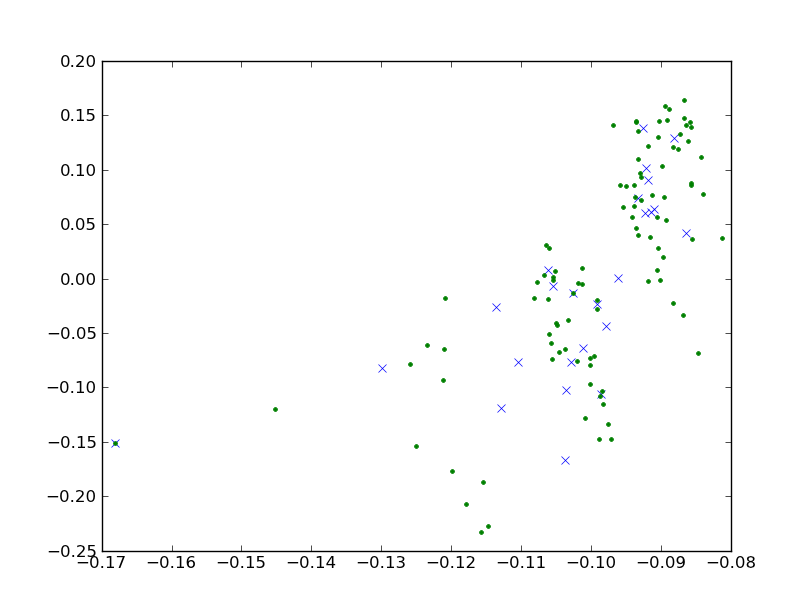
\includegraphics[height=8cm]{wordsvd.png}

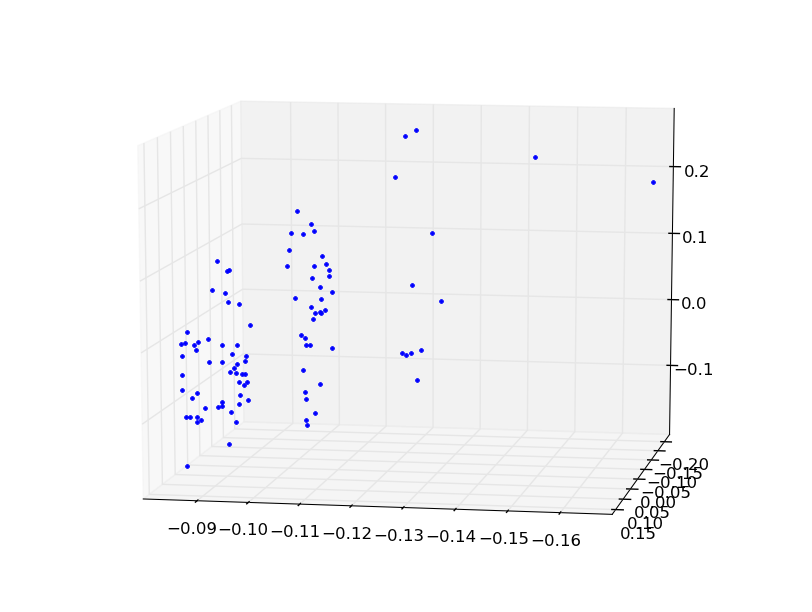
\includegraphics[height=8cm]{wordsvd3.png}

Sonuc

\begin{verbatim}
this
['this' 'think']
by
['a' 'I' 'as' 'by' 'my' 'up' 'us']
back
['say' 'all' 'can' 'also' 'back' 'want' 'day']
your
['out' 'about' 'your' 'our']
there
['there' 'their' 'these']
will
['with' 'will' 'which']
for
['of' 'for' 'not' 'you' 'or']
could
['would' 'people' 'could']
get
['at' 'but' 'her' 'get' 'year']
be
['be' 'he' 'we' 'she' 'me' 'see' 'use' 'new']
like
['like' 'time' 'give']
do
['to' 'do' 'so' 'go' 'no' 'two' 'how']
its
['in' 'it' 'his' 'if' 'him' 'into' 'its']
who
['who']
one
['on' 'one' 'only' 'even']
some
['some' 'come']
when
['when' 'well']
just
['just' 'first' 'most']
what
['that' 'what' 'way']
they
['the' 'they' 'them' 'than' 'then']
good
['from' 'know' 'good' 'now' 'look' 'work']
have
['have' 'make' 'take']
over
['other' 'over' 'after']
because
['because']
any
['and' 'an' 'any']
\end{verbatim}

Bu teknigin uygulanabilecegi daha pek cok alan var. Mesela her dokumanin
icindeki belli kelimelerin sayilari kolonlarda (her kolon ozel bir kelimeye
tekabul edecek sekilde), ve dokumanlarin kendisi satirlarda olacak sekilde
bir matrisimiz olsaydi, SVD bu matris uzerinde de bir kumeleme icin
kullanilabilirdi. Bu ornekte ``kac tane kelime oldugu'' gibi bir olcut
vardir (daha once kelimelerin birbirine uzakligini kullandik), ama teknik
yine de ise yarar.

[1] http://kdd.ics.uci.edu/databases/synthetic\_control/synthetic\_control.data.html

[2] http://sayilarvekuramlar.blogspot.de/2012/07/kelime-benzerligi-levenshtein-mesafesi.html

[3] Skillicorn, D., {\em Understanding Complex Datasets Data Mining with Matrix Decompositions}


\end{document}
